\documentclass{beamer}
\mode<presentation>
\usetheme{CambridgeUS}
\usecolortheme{beaver}
\setbeamertemplate{caption}[numbered]

\usepackage[english]{babel}
\usepackage{graphicx}
\usepackage{subfigure}
\usepackage{url}
\usepackage[backend=bibtex, style=verbose]{biblatex}
\usepackage{multicol}
\bibliography{bibliography.bib}
\usepackage[noend]{algorithm,algpseudocode}


\title[Depth Estimation]{Depth Estimation Using Deep Neural Networks}
\author[Mu\c sat Bogdan-Adrian]{Mu\c sat Bogdan-Adrian}
\date{December 2017}

\beamertemplatenavigationsymbolsempty
\graphicspath{{./images/}}

\begin{document}

\frame{\titlepage}

\begin{frame}
\frametitle{Problem Formulation}
\center
\begin{itemize}
	\item Given a pair of stereo images, how to estimate the depth of the existing objects?
\end{itemize}
\end{frame}

\begin{frame}
\frametitle{Disparity}
\center
\begin{itemize}
	\item Disparity represents the difference of perspective created by the horizontal or vertical separation of two cameras
	\item The human brain processes disparity information from both eyes to estimate the depth of real world objects
	\item Disparity is inverse proportional with depth; given the basline distance \(b\) between the cameras and the camera focal lenght \(f\), the depth \(\hat{d}\) from the predicted disparity \(d\) is simply \(\hat{d}=bf/d\)
	\item Objects closer to the camera have bigger disparities, whilst objects that are farther have smaller disparities
\end{itemize}
\end{frame}

\begin{frame}
\frametitle{Proposed Solution}
\center
\begin{itemize}
	\item Given a pair of rectified \footnote{Vertically aligned} stereo images as input, build a model which can accurately predict the disparity per-pixel (i.e. learn the \(\Delta\) values with which every pixel from the left image is shifted from the right one on the \(x\) axis)
	\item Such a system can be modeled by a Convolutional Neural Network
\end{itemize}
\end{frame}

\begin{frame}
\frametitle{Challenges - Textureless Areas}
\center
\begin{itemize}
	\item Depth estimation is an ill-posed problem: a pixel in a textureless area from the left image can belong to multiple pixels in the right image
\end{itemize}
\begin{figure}
    \centering
        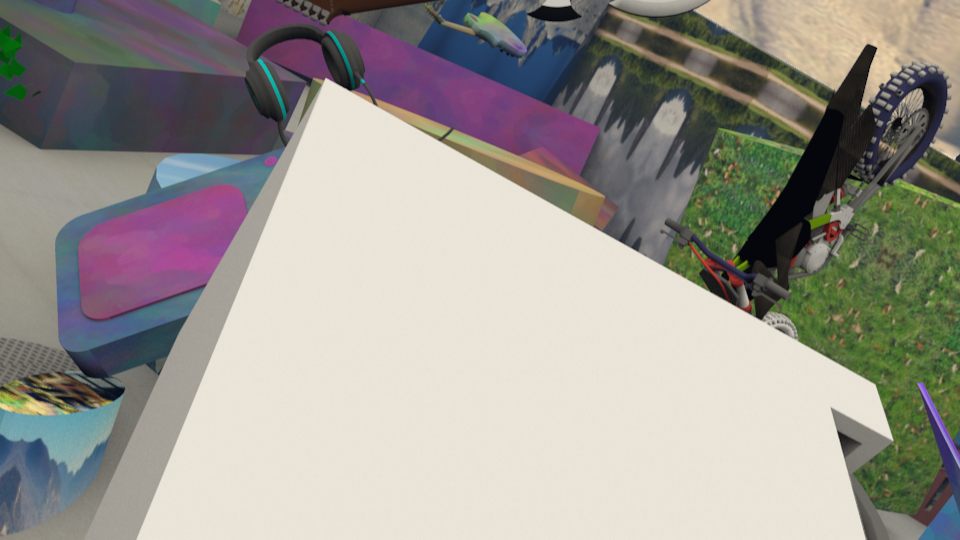
\includegraphics[width=0.6\textwidth]{textureless.png}
        \caption{Example of objects with textureless areas}
    \end{figure}
\end{frame}

\begin{frame}
\frametitle{Challenges - Object Occlusion}
\center
\begin{itemize}
	\item Parts of an object may be visible in an image, while being absent in the other one because of the difference of perspective
\end{itemize}
\begin{figure}
	\centering
	\begin{subfigure}
		\centering
    	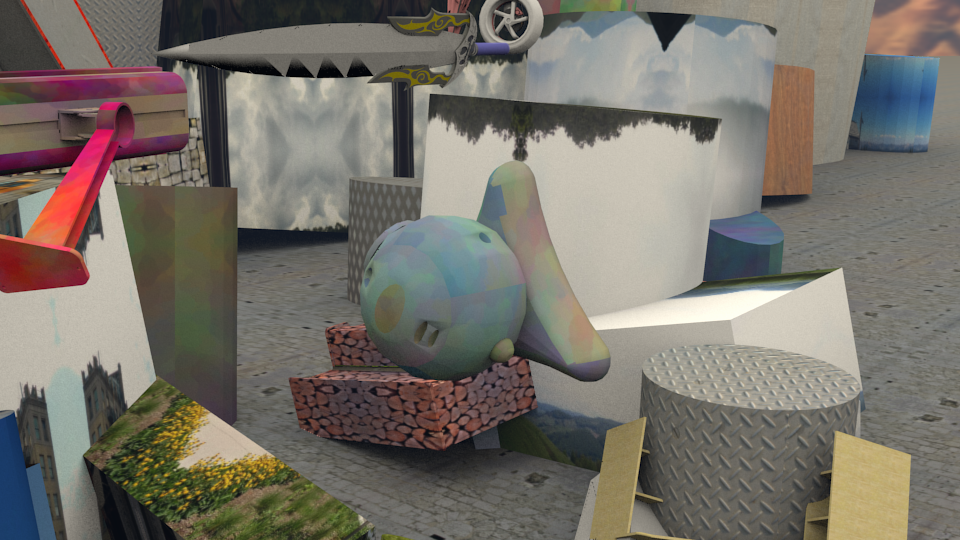
\includegraphics[width=0.45\textwidth]{occlusion_left.png}
    \end{subfigure}
    \begin{subfigure}
		\centering
        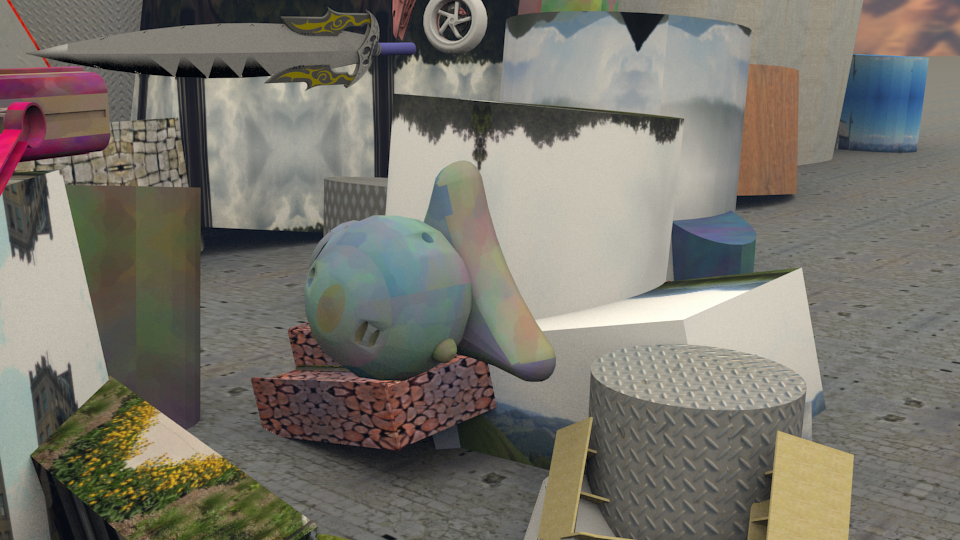
\includegraphics[width=0.45\textwidth]{occlusion_right.png}
    \end{subfigure}
    \caption{Occlusion in stereo images}
\end{figure}
\end{frame}

\begin{frame}
\frametitle{Convolutional Neural Networks Architectures}
\center
\begin{itemize}
	\item Supervised
		\begin{itemize}
			\item Requires ground-truth disparity, which might be expensive to obtain
			\item Based on disparity regression
			\item Accurate predictions
		\end{itemize}
	\item Unsupervised
		\begin{itemize}
			\item Does not require any form of ground-truth
			\item Based on an image reconstruction loss
			\item Has artefacts around the edges of objects, caused by occlusion
		\end{itemize}
\end{itemize}
\end{frame}

\begin{frame}
\frametitle{DispNet\footcite{DBLP:journals/corr/MayerIHFCDB15} - Overview}
\center
\begin{itemize}
	\item Image-to-image autoencoder structure
\end{itemize}
\begin{figure}
    \centering
        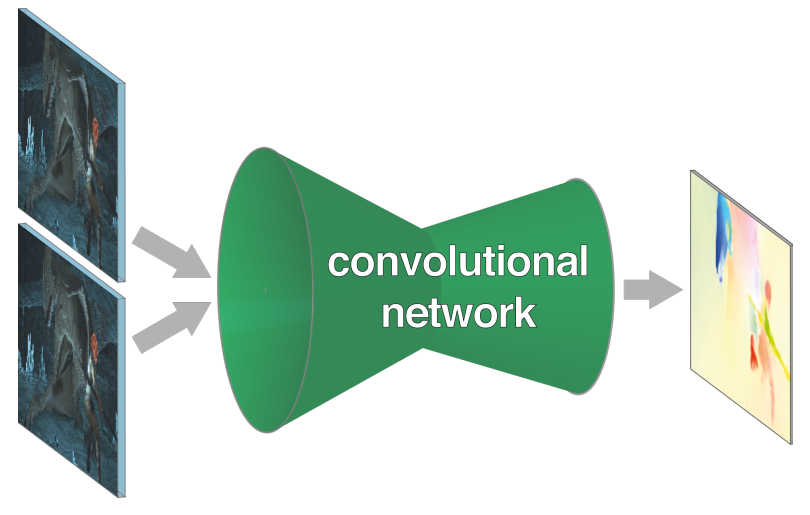
\includegraphics[width=0.5\textwidth]{hourglass.png}
        \caption{Hourglass structure of DispNet}
    \end{figure}
\end{frame}

\begin{frame}
\frametitle{DispNet - Architectural Details}
\center
\begin{itemize}
	\item Fully Convolutional Network\footcite{DBLP:journals/corr/LongSD14}
	\item Concatenates the ``upconvolution'' results with the features from the ``contractive'' part to recover spatial information lost by downsampling
	\item Uses smooth L1 loss between the resulted disparity computed at different pyramid levels of the network and the ground-truth
	\[
	\lvert d \rvert _{smooth}=
	\begin{cases}
	0.5d^2, & if \lvert d \rvert \leq 1\\
	\lvert d \rvert -0.5, & otherwise\\
	\end{cases}
	\]
\end{itemize}
\end{frame}

\begin{frame}
\frametitle{DispNet - Architectural Details}
\center
\begin{itemize}
	\item The upsampling part of the network can be constructed by using transposed convolutions\footcite{Zeiler:2011:ADN:2355573.2356530} or by using interpolation methods like nearest neighbor or bilinear followed by a convolutional layer to smoothen the results
\end{itemize}
\end{frame}

\begin{frame}
\frametitle{DispNet - Results}
\center
\begin{figure}
	\centering
	\begin{subfigure}
		\centering
    	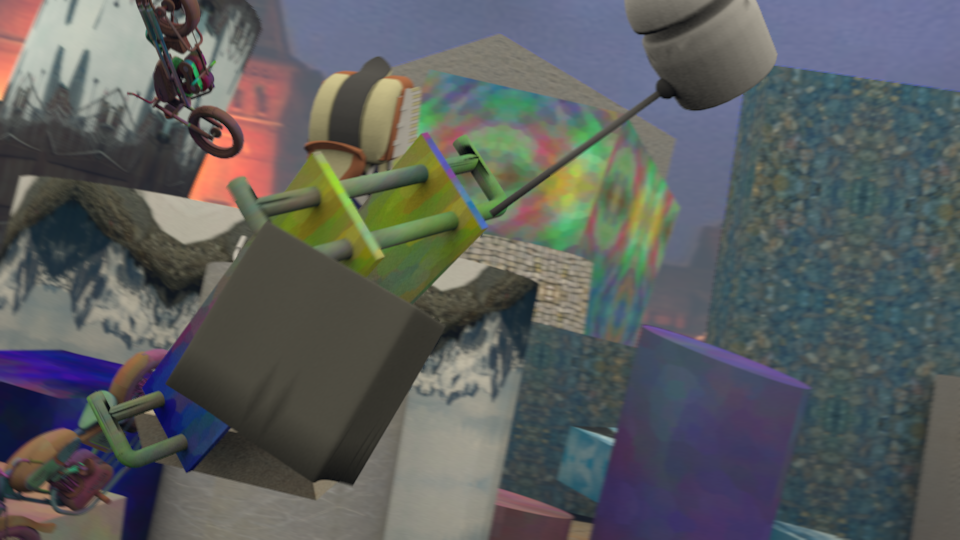
\includegraphics[width=0.45\textwidth]{original_depth.png}
    \end{subfigure}
    \begin{subfigure}
		\centering
        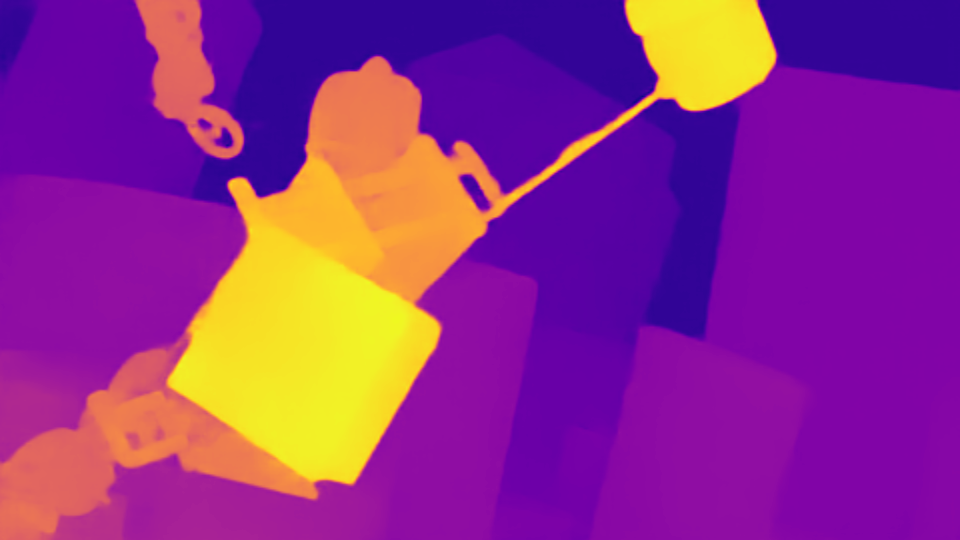
\includegraphics[width=0.45\textwidth]{dispnet_estimation.png}
    \end{subfigure}
    \caption{Supervised depth estimation}
\end{figure}
\end{frame}

\begin{frame}
\frametitle{Unsupervised Monocular Network\footcite{DBLP:journals/corr/GodardAB16} - Overview}
\center
\begin{itemize}
	\item Similar architecture as DispNet
\end{itemize}
\begin{figure}
    \centering
        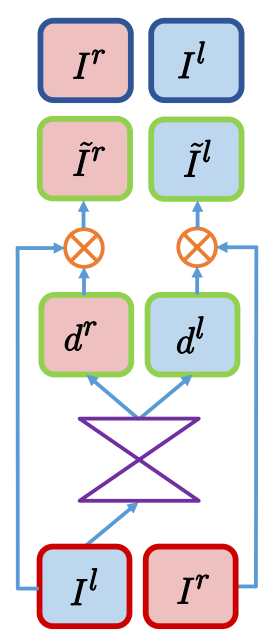
\includegraphics[width=0.2\textwidth, height=0.5\textheight]{monodepth.png}
        \caption{Unsupervised Monocular Network architecture}
    \end{figure}
\end{frame}

\begin{frame}
\frametitle{Unsupervised Monocular Network - Architectural Details}
\center
\begin{itemize}
	\item Shares the same hourglass structure as DispNet and works the same, up until a point
	\item Instead of using ground-truth disparity, the network tries to reconstruct the right image from the left one, and vice-versa
	\item The network tries to achieve the needed disparities as to warp the left and right image using some sampling method
	\item The sampling method chosen is binilinear sampling as used in Spatial Transformer Networks\footcite{DBLP:journals/corr/JaderbergSZK15}, which is fully differentiable
	\item Produces disparity estimates at four scales
\end{itemize}
\end{frame}

\begin{frame}
\frametitle{Unsupervised Monocular Network - Architectural Details}
\center
\begin{itemize}
	\item Uses a three term loss
	\[
		C_s=\alpha_{ap}(C^l_{ap}+C^r_{ap})+\alpha_{ds}(C^l_{ds}+C^r_{ds})+\alpha_{lr}(C^l_{lr}+C^r_{lr})
	\]
	\item Appearance Matching Loss
	\[
		C^l_{ap}=\frac{1}{N}\sum_{i,j}\alpha\frac{1-SSIM(I^l_{ij},\tilde{I}^l_{ij})}{2}+(1-\alpha)\lVert I^l_{ij}-\tilde{I}^l_{ij}\rVert
	\]
	\item Disparity Smoothness Loss
	\[
		C^l_{ds}=\frac{1}{N}\sum_{i,j} \lvert \partial_x d^l_{ij} \rvert e^{-\lvert \partial_x I^l_{ij} \rvert} + \lvert \partial_y d^l_{ij} \rvert e^{-\lvert \partial_y I^l_{ij} \rvert}
	\]
	\item Left-Right Disparity Consistency Loss
	\[
		C^l_{lr}=\frac{1}{N}\sum_{i,j} \lvert d^l_{ij} - d^r_{ij + d^l_{ij}} \rvert
	\]
\end{itemize}
\end{frame}

\begin{frame}
\frametitle{Unsupervised Monocular Network - Results}
\center
\begin{figure}
	\centering
	\begin{subfigure}
		\centering
    	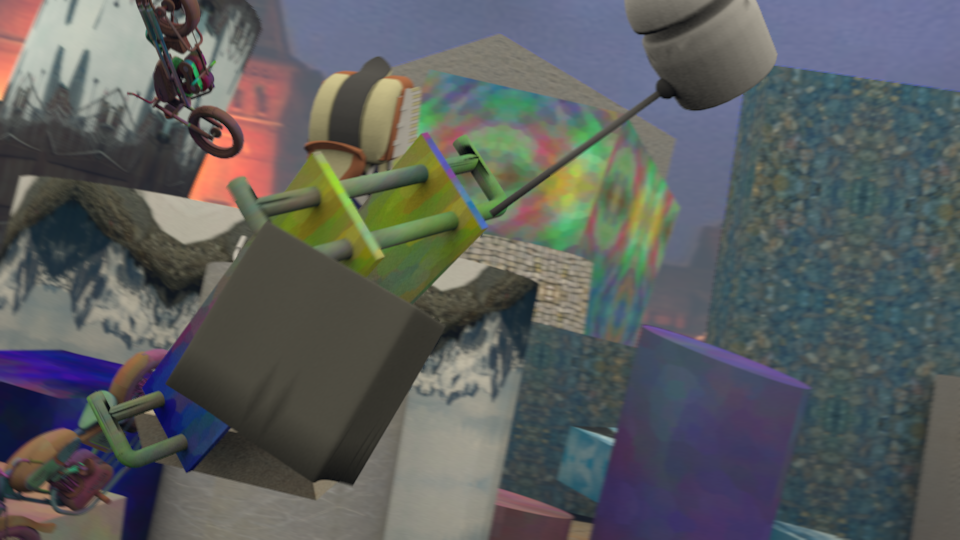
\includegraphics[width=0.45\textwidth]{original_depth.png}
    \end{subfigure}
    \begin{subfigure}
		\centering
        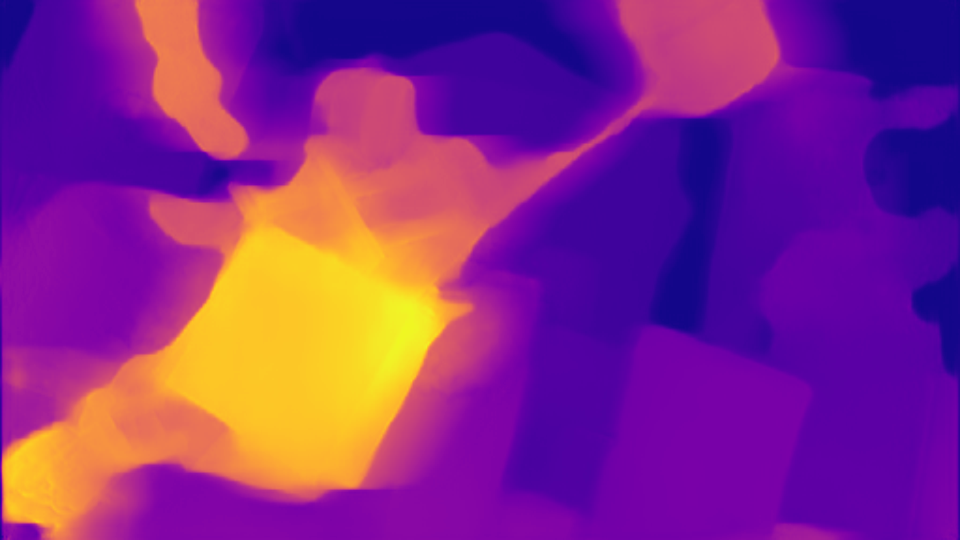
\includegraphics[width=0.45\textwidth]{monodepth_estimation.png}
    \end{subfigure}
    \caption{Unsupervised depth estimation}
\end{figure}
\end{frame}

\end{document}
